
\documentclass{scrartcl}

\usepackage{hyperref}
\usepackage{graphicx}

\title{Custom Padding on the HEALPix Geometry}
\author{Matthias Karlbauer}

\begin{document}
	\maketitle
	
	\paragraph{HEALPix} The Hierarchical Equal Area isoLatitude Pixelization (HEALPix) is a geometric representation of a sphere with several neat properties \cite{gorski2005healpix}. It separates a sphere into twelve faces, defining respectively four fields to represent the north-, equator-, and south-regions. A visualization of the twelve faces approximating the sphere is given in \autoref{fig:face_order}.
	
	\begin{figure}
		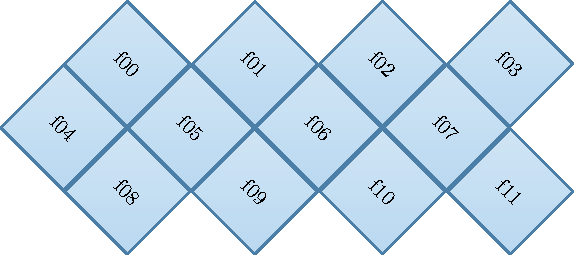
\includegraphics[width=\linewidth]{pics/face_order}
		\caption{Arrangement of the twelve faces defining the HEALPix. The diamond shapes fold together horizontally to approximate a sphere.}
		\label{fig:face_order}
	\end{figure}
	
	\paragraph{Deep Learning on the HEALPix} In order to apply convolutions on the HEALPix geometry, a customized padding operation needs to be implemented. This will guarantee the correct information propagation among neighboring faces. North and south faces can be implemented straight forward under consideration of rotating certain neighbor faces.
	
	Equatorial faces require a particular treatment of the neighbors at their north and south corners (or top-left and bottom-right from a face-centric view). A detailed neighborhood description for each face is outlined in \autoref{fig:padding}. More explanations considering the particular treatment of the equatorial top-left and bottom-right neighbors are given in \autoref{fig:corners}.
	
	\begin{figure}
		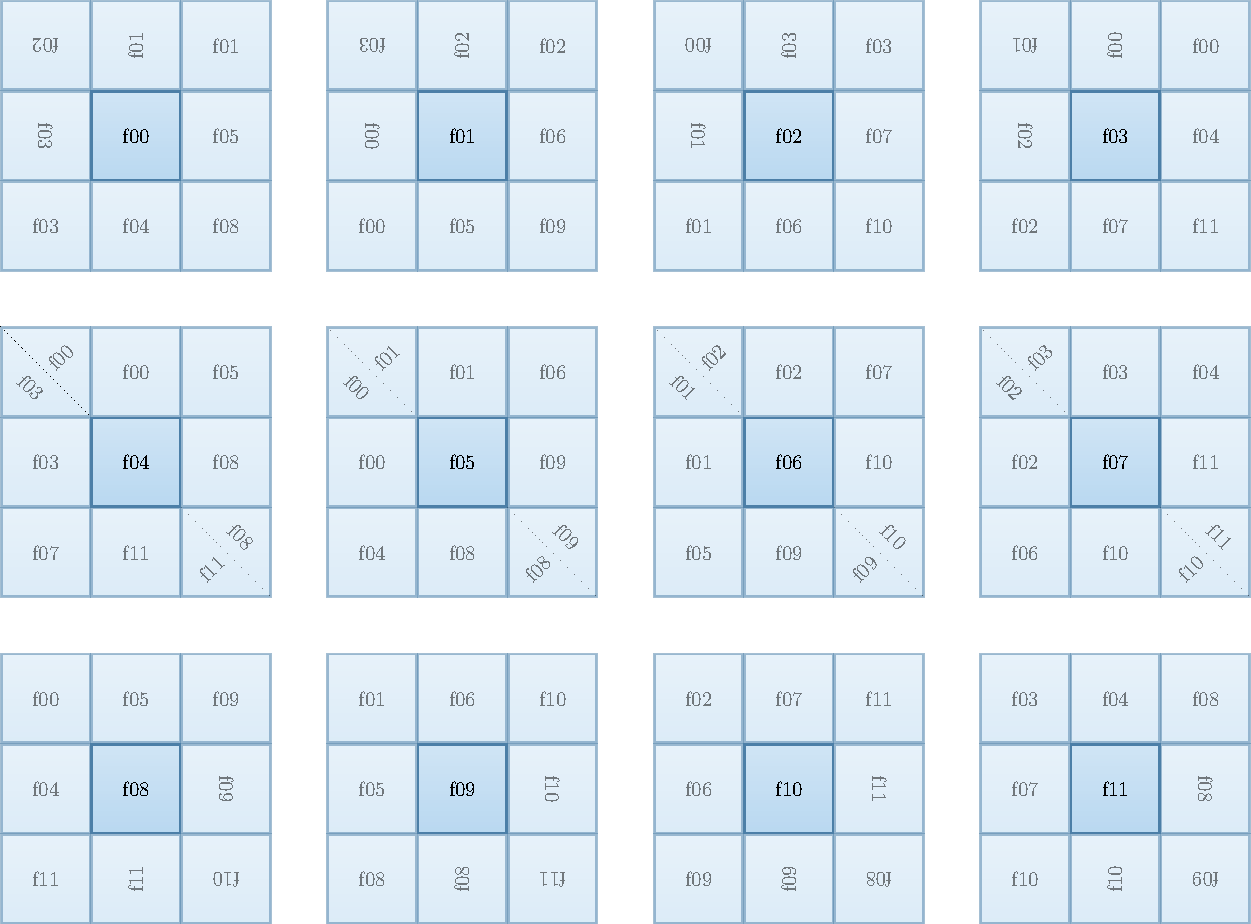
\includegraphics[width=\linewidth]{pics/padding}
		\caption{Neighboring faces and their orientation with respect to each `center' face of the HEALPix. First row: north faces, second row: equator faces, third row: south faces.}
		\label{fig:padding}
	\end{figure}

	\begin{figure}
		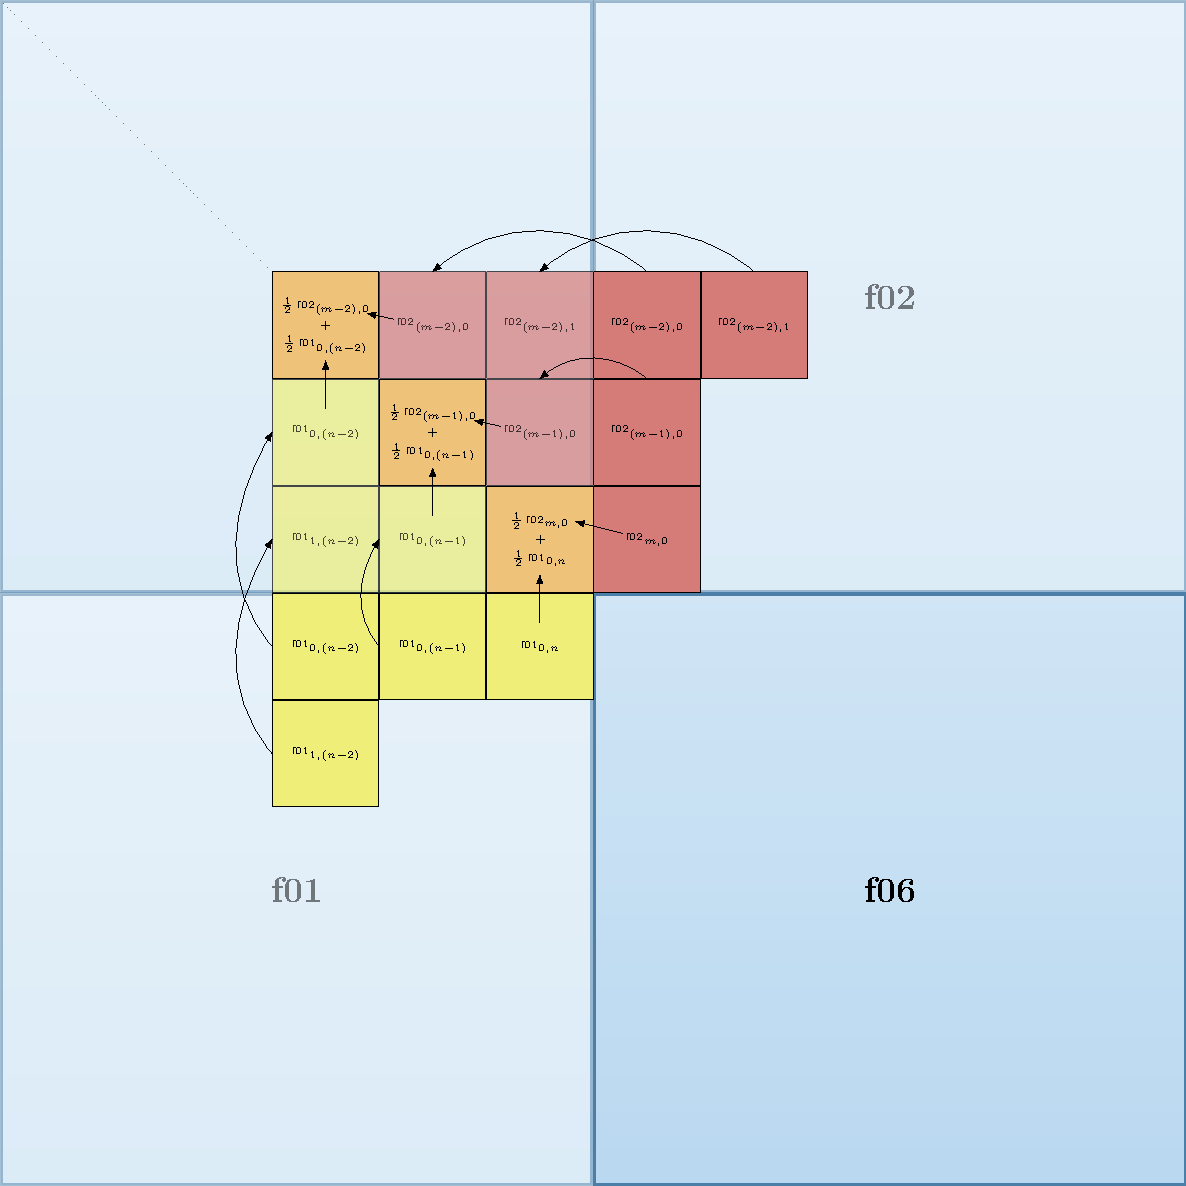
\includegraphics[width=\linewidth]{pics/corners}
		\caption{Treatment of the top-left corner of the exemplary equator face f06. Orange colored entries on the diagonal are interpolated (effectively averaged) from the neighbors (intuitively rotated by $\pm45^\circ$, as shown in \autoref{fig:face_order}), whereas values off the diagonal are taken directly from the according neighbors (yellow and red). The procedure for the bottom-right corner is defined analogously.}
		\label{fig:corners}
	\end{figure}
	\bibliographystyle{unsrt}  
	\bibliography{literature}
\end{document}